\Chapter{Komponensek}
\label{Chap:komponensek}

\section{Felhasznált technológiák (C++, SDL)}

Windows operációs rendszeren az általam legjobban megkedvelt program a Microsoft Visual Studio, aminek a 2015-ös verzióját használom. Az évek során nagyon megszoktam a kezelőfelületét, illetve az azon elhelyezkedő gombok, funkciók elérhetősége ebben a leglogikusabbak számomra. A játék megírásához számomra a C++ programozási nyelv tűnt a legmegfelelőbbnek. A mai játékok jó része is ezzel a nyelvvel íródik, mivel „natív” fut a kód a gépen, sokkal jobb választás mint a C\# vagy a Java. Ezalatt azt értem, hogy például egy Java nyelven megírt program futtatásához szükség van egy virtuális gépre, ami tudja értelmezni a fordító által lefordított, még nem gépi kódot. A virtuális gép felelős azért, hogy az adott hardver gépi kódjára forduljon a program. Vannak olyan alkalmazási területek, ahol az utóbbi kettő a jobb, de egy játék esetében az a lényeg minél gyorsabban fusson egy adott gépen, minél több FPS-t (képkocka/másodperc) produkálva.

A képi világ kirajzolásához, illetve a hangok megszólaltatásához az SDL 2.0-t választottam. Az alábbi linken található bővebb leírás, hogy mit is takar pontosan az SDL:

\begin{verbatim}
https://hu.wikipedia.org/wiki/Simple_DirectMedia_Layer
\end{verbatim}

\section{Az alkalmazás fő részei}

A fő részek, és azok kapcsolatainak szemléltetéséhez egy osztálydiagramot készítettem. Ezen megtekinthető a játék felépítése, melyik osztálynak melyik az őse, illetve mely osztályok vannak kapcsolatban egymással. Továbbá feltüntetésre kerültek a kapcsolatokhoz szükséges adattagok, vagy metódusok is.

Ahogy \aref{fig:uml}-es ábrán is látható, a MainGame a játék fő osztálya, ehhez kapcsolódik minden egyéb komponens, és ez felel az ablak inicializálásáért, felhasználói interakciók lekezeléséért. A játékbeli interakciók kezeléséért az Action osztály felelős, ez kezeli az állapotokat, például hogy éppen előre vagy hátra haladunk, ugrunk, vagy futunk. Ennek megfelelően az Action osztály kimenetei alapján a Player végzi el a játékoshoz kapcsolódó cselekvéseket. A MainGame-hez kapcsolódik még közvetlen a Map, a Sound, a MainMenu osztály. 

A Map a játéktér elemeit, és az azokkal kapcsolatos dolgokat foglalja össze. Ide kapcsolódik a DrawHeightMap, amin keresztül betölti, kirajzolja a játék alapját képző domborzatot, és kiszámolja a karakter ütközésvizsgálatához szükséges gradienst is. A VboDrawer és őse a ModelLoader az egyéb játékbeli objektumok (fák, tárgyak) betöltéséért, kirajzolásáért felelős. A BulletCalcs3D a lövéshez kapcsolódó háttérszámításokat végzi, és az adott háromszöggel kapcsolatos x,y,z metszéspontot adja vissza. A Materials osztály az anyagjellemzők beállításáért felelős.

A játék részeit képezik a játékos informálásáért és segítéséért felelős 2D-s elemek is, amelyekért az IngameElements3D osztály felelős. Ez jeleníti meg a célkeresztet, rajzolja ki az életerő és a lőszer mennyiséget jelző textúrát is, amelyeket viszont a Texture osztály tölt be.

A MainMenu osztályban a főmenühöz kapcsolódó elemek vannak, amelyek a menü háttere, illetve a kijelölések lekezelése vizuálisan. Ezeket az elemeket is a VboDrawer és őse a ModelLoader tölti be, rajzolja ki.

A Sound a hangok megszólalásáért, a megfelelő zenék lejátszásáért felelős, az Utils pedig az egyéb, többi osztályba nem tartozó elemeket tartalmazza.

\begin{figure}[h]
\centering
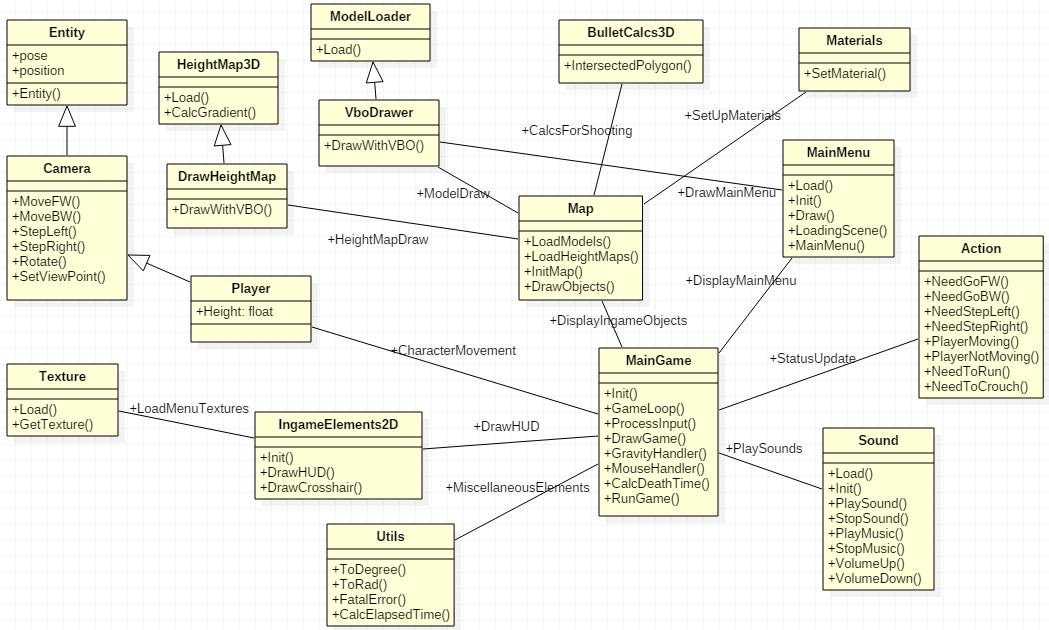
\includegraphics[scale=0.5]{kepek/uml.png}
\caption{A játék felépítése}
\label{fig:uml}
\end{figure}

\subsection{Magasságmező-betöltés, textúrázás}

A játék .obj kiterjesztésű modelleket használ, és ezekre húzza rá a textúrát. A megjelenítéshez VBO-t, azaz Vertex Buffer Object-et használ, ami a modell adatait tárolja, és egyben, a legmegfelelőbb formátumban adja át a videókártyának az optimális sebességért.

Ez egy fekete fehér kép 256 színárnyalatából tud 256 különböző magasságértéket számolni. Mint ahogy korábban is említésre került, a fekete a legalacsonyabb, a fehér a legmagasabb terület, így könnyedén lehet hegyeket illetve völgyeket kialakítani. A játék játszható területének megadásához például \aref{fig:heightmap} ábrán látható képet adhatjuk meg, amiből a magasság értékek számolódnak. A magasságmező textúráját egy külön képfájlból tölthetjük be. Egy ilyen látható \aref{fig:heightmap_texture} ábrán.

\begin{figure}[h]
\centering
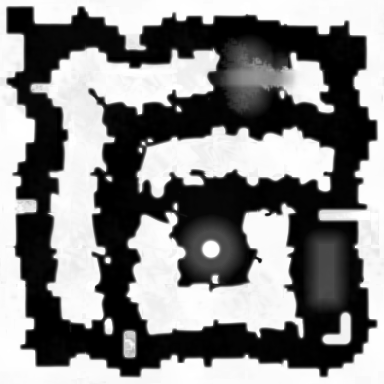
\includegraphics[scale=0.5]{kepek/heightmap.png}
\caption{A magasságmező adatait tartalmazó bitmap}
\label{fig:heightmap}
\end{figure}

\begin{figure}[h]
\centering
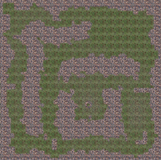
\includegraphics[scale=1.5]{kepek/heightmap_texture.png}
\caption{A magasságmező textúrája}
\label{fig:heightmap_texture}
\end{figure}

\Aref{fig:screenshot} képen pedig a játékban való megjelenés látható. Ez egyben megoldja az ütközéskezelést is, illetve, hogy a túl meredek parton ne lehessen felmenni (lecsúszik róla). A pontokat lineárisan interpolálja, ezzel alkot összefüggő felületet. A textúra ráillesztése is problémás lehet a magasságmezőre, mivel olyan helyeken, ahol túl nagy a gradiens, elnyújtódik. Erre megoldás lehet a multitextúrázás.

\begin{figure}[h]
\centering
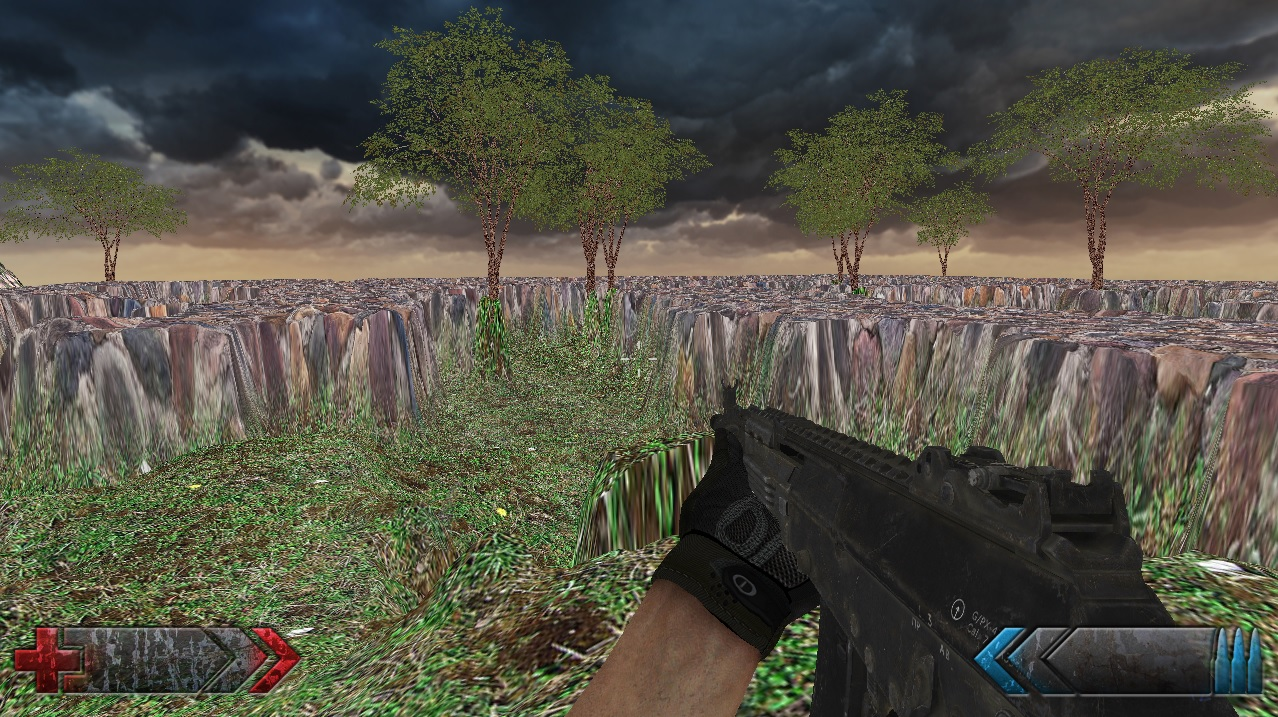
\includegraphics[scale=0.4]{kepek/screenshot.png}
\caption{A megjelenített magasságmező}
\label{fig:screenshot}
\end{figure}

\subsection{A karakter irányítása, fizika}

A játékban egy karaktert irányíthatunk az ő szemszögéből. A karakternek van magassága, x,y,z pozíciója, nézési iránya, amit lát, vagy látunk, a játék szempontjából egy kamera. A kamerához van forgatva a fegyvere, és az ő szemszögéből látható testrészei. Minden cselekedetéhez tartozik egy bool (két állapotú) változó. Például ha tegyük fel előre megyünk, akkor az ehhez tartozó változó „true (igaz)” értéket vesz fel, amihez különböző eseményeket lehet kötni, mint például a kamera előre mozgatását, bizonyos animációk lejátszását. Továbbá a játékosra folyamatosan hat egy gravitációs erő, ami egy float típusú szám. Ezzel lehet elérni azt, hogy ha ugrunk, a játékos visszaessen a talajra.

\subsection{Hangok}

Egyidejűleg több hang lejátszására is szükség lehet, amelyet valamilyen események váltanak ki. A karakter előrehaladása közben egyidejűleg ha lövünk is, már több hangcsatornát igényel, mert így nem várja meg a két hang egymást. Ha csak egy csatorna van, akkor a lépéshangot lejátssza, és csak ez után hallhatjuk a lövést, ami frusztráló, és nem reális. Mivel a játékmenet közben egy hangulatfokozó zene is hallható, ennek lejátszásához, a lépéshanghoz és a lövéshez máris három hangcsatornára van szükség. 

\begin{figure}[h]
\centering
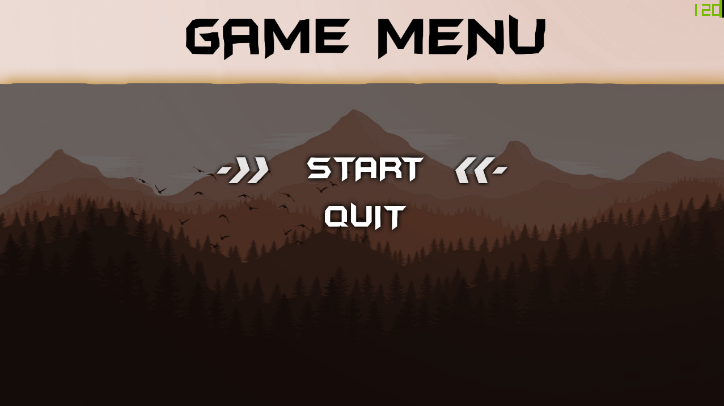
\includegraphics[scale=1.6]{kepek/menu.png}
\caption{A főmenü}
\label{fig:menu}
\end{figure}

\begin{figure}[h]
\centering
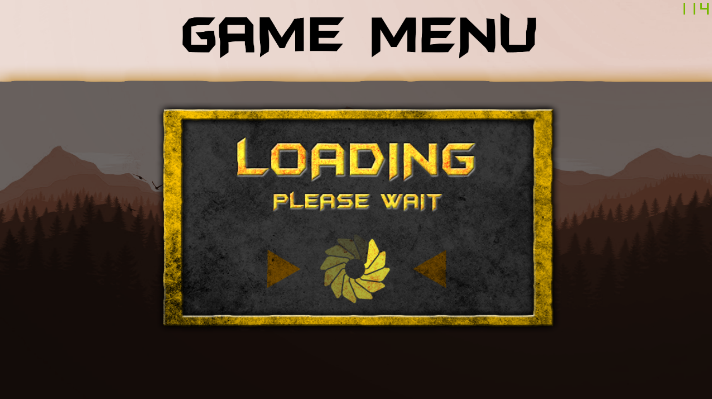
\includegraphics[scale=1.6]{kepek/loading_screen.png}
\caption{Pályabetöltés közben ez látható}
\label{fig:loading}
\end{figure}

\subsection{Lövés}

A lövés háttérszámításai, matematikai kalkulációk is egy külön komponensnek tekinthetők. Első lépés, hogy ki kell számolni a vektort amerre a játékos néz, minden képkockára. Mivel a világ háromszögekből épül fel, ezért ki kell számolni az egyenes háromszöggel való metszéspontját. De mivel több százezer háromszögről beszélünk, ez további optimalizálandó problémákat vet fel, amit a későbbiekben fejtek ki. Bemeneti adatai a játékteret képző háromszögek, illetve a játékos irányvektora, kimeneti adatai pedig a metszéspont x,y,z koordinátája.

\subsection{Mesterséges intelligencia}

Egyjátékos FPS játékról van szó, így mindenféleképp kellett egy, az ellenfelek mozgását irányító mesterséges intelligencia. Ez az egész az A* algoritmusra alapszik. A játék véletlenszerűen, különböző helyekre kirak x mennyiségű ellenfelet, amiknek közeledni kell a játékos felé, különböző kritériumoknak megfelelve. Ezek a kritériumok azért kellenek, mert a pályán vannak játékelemek, amiken nem lehet átmenni, illetve az ellenfelek sem mehetnek egymásba. 

Az alapötlet az, hogy a pályán le lesznek rakva pontok, ún. waypointok, amik csak az ellenfelek számára lesznek láthatók. Ha kikerül egy adott ellenfél a pályára, az első feladata az lesz, hogy megkeresse a hozzá legközelebb eső waypointot. Ezután az A* algoritmus segítségével meghatározza a játékoshoz legközelebb eső waypointhoz vezető legrövidebb utat, végigmegy rajta, majd ha elérte, akkor onnantól a játékos lesz a közvetlen elsődleges célpontja. Mivel a játékos folyamatosan mozog, mindezt másodpercenként legalább 15-30x kell kiszámolni.

Bemeneti adatai a waypointok azok típusaival együtt, kimeneti adata pedig az adott útvonal, hogy az ellenfélnek merre is kell mozognia. Az ellenfél elsődleges célpontja a játékos, de adódhatnak olyan helyzetek amikor előtte egyéb dolgokat helyez előtérbe, mint például az életerő töltés, vagy lőszer felvétel. Itt fontos szerepet kap az ellenfél karakterisztikája, ami szintén bemeneti paraméter.


\section{A játékindítás folyamata}

Első lépésben a játék létrehozza az SDL ablakot, és konkrétan beállítja annak pozícióját, függőleges és vízszintes felbontását, illetve a flageket, pl. a kurzort, teljes képernyő legyen vagy nem.

A második lépés hogy az előtte létrehozott ablakot beállítja aktívra, és OpenGL megjelenítésre. Létre kell hozni egy érvényes OpenGL  kirajzolás kontextust, hogy inicializáljuk a belépési pontokat. Ez használhatóvá teszi az összes elérhető funkciót, amit az OpenGL magban definiáltak. Ezután betölti a főmenü megjelenítéséhez szükséges modelleket, textúrákat.

Harmadik lépésben aktiválja a hangok megszólaltatásáért felelős komponenst, és betölti az összes hangot, zenét.

A negyedik lépésben pedig aktiválja az eseménykezelő komponenst, ami a felhasználótól érkező interakciókat kezeli, majd meghívja a betöltött modelleket kirajzolásra.

A menübe érkezés után a felhasználónak lehetősége nyílik a játékteret betölteni, vagy kilépni. 

A „Start” gombra kattintás után, betöltődik a magasságmező kezelő komponens, a kamera a kezdőpontra pozícionálódik, elkezdődnek a játékmenethez elengedhetetlen háttérszámítások, és egy új zene lejátszása, betöltődnek a játéktér modelljei, elemei, illetve átvált azok kirajzolására. Hogy a játékos informálva legyen, ez idő alatt megjelenik a betöltőképernyő.

\begin{figure}[h]
\centering
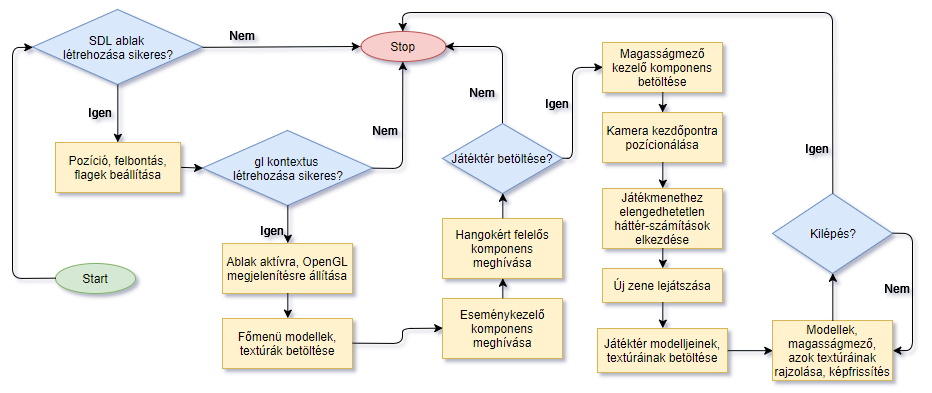
\includegraphics[scale=0.46]{kepek/starting_diagram.png}
\caption{A játék indításának folyamatábrája}
\label{fig:starting}
\end{figure}